\chapter*{About provable reproducibility}
\label{chp:0-reproducibility}

How can scientists unmistakably know whether their results can be reproduced
by other people? How can reviewers quickly verify that a certain numerical
experiment in an article is correct? And how can collaborators quickly
understand how to use the source code you have written for your project?\\

Provable reproducibility is an initiative I hereby launch, which pursues the
goal of making results published in articles, theses, and software packages easier to
reproduce and verify. No more ambiguity, misunderstandings, cherry-picked
parameters, and hand-crafted results. Every figure, plot, and table
in a provably reproducible project can be unequivocally traced back to where
it originated from. This goes one step further than the practice of open-sourcing
the code of a project, where a reviewer or user still has to go through the
tedious and often error-prone process of reproducing your results.\\

Like in a public demonstration of a scientific experiment, the proof is delivered
by remotely -- not locally -- recreating every aspect of a project, for example
in an online archive. Everyone can see what steps are taken to achieve a certain outcome.
Making a project provably reproducible includes, but is not limited to,
explicitly downloading, importing, and building all the external dependencies which are being used (code, data, \dots);
running all the computations and generating the corresponding results (plots, tables, \dots);
and compiling the project outcome (article, report, \dots).
A reproducibility proof can be achieved without too much effort by
using the continuous integration frameworks offered in most contemporary
software development and version control services, such as GitHub actions or
GitLab CI/CD. Corresponding guidelines and resources will be made available in due
time\footnote{\url{https://github.com/FMatti/Re-Pro}}.

\begin{center}
    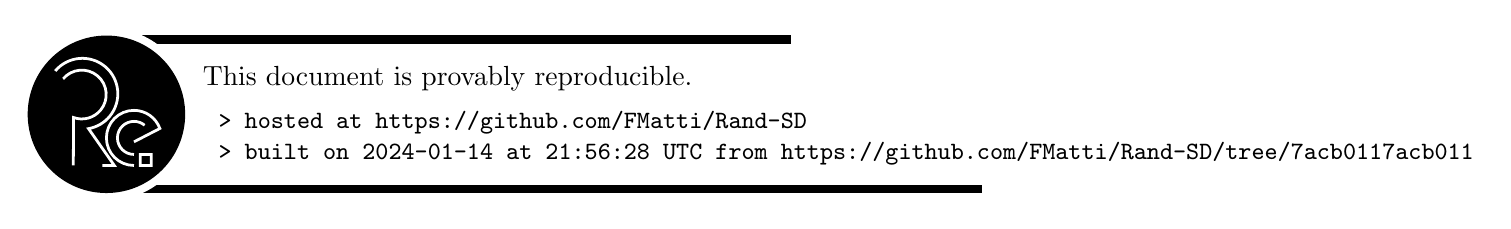
\begin{tikzpicture}
    \draw[black, line width=3pt] (0.1, 0.95) to (0.8\textwidth, 0.95) (0.1, -0.95) to (\textwidth, -0.95);
    \fill[white] (0, 1.1) to (1, 1.1) arc (90:-90:1.1) to (0, -1.1);
    \fill[black] (1, 0) circle (1);
    \draw[white, line width=1pt] (0.35, 0.55) arc(140:-80:0.45) to (1.1, -0.65) to (0.95, -0.65) (0.45, 0.45) arc(140:-110:0.31) to (0.58, -0.65) (1.35, -0.65) arc(270:20:0.35) to (1.35, -0.35) (1.35, -0.51) arc(270:50:0.21) (1.43, -0.65) rectangle (1.57, -0.51);
    \node[anchor=west] at (2.1, 0.45) {This document is provably reproducible.};
    \node[anchor=west] at (2.3, -0.1) {\small \texttt{> hosted at \url{https://github.com/FMatti/Rand-SD}}};
    \node[anchor=west] at (2.3, -0.5) {\small \texttt{> built on 2024-01-14 at 21:56:28 UTC from \href{https://github.com/FMatti/Rand-SD/tree/7acb011}{7acb011}}};
\end{tikzpicture}

\end{center}
